\label{sec:intro}
\section{Analysis of Texture in Scene Images}

%It also provides a rich source of information about the
%natural scene and hence 
Texture refers to a surface characteristic and appearance of an object given by
its geometry, density and surface reflectance, and the stochastic variation of
these parameters.
It is a detailed pattern that is mapped into a multidimensional space.
It is an important cue in trying to achieve photorealistic
rendering of 3D models by adding surface details or color to an object or a
scene. Some of the natural scene textures are shown in Fig \ref{fig:texture}

3D Texture modelling is an important area in computer graphics as it results in realistic rendering
of natural material surfaces. The characterization of surface reflectance properties is important in
achieving photorealism. The appearance of a surface in different lighting and viewing direction/conditions 
is affected by its reflectance properties. 3D texture actually models the relation
between surface reflectance properties and illumination direction.

\begin{figure}[t]
\centering
\subfigure{

\includegraphics[height=1.5in,width=1.8in]{texture/1.eps}
}
\subfigure{

\includegraphics[height=1.5in,width=1.8in]{texture/2.eps}
}
\subfigure{
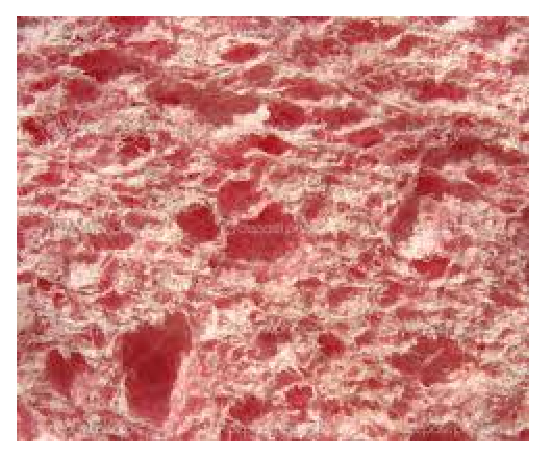
\includegraphics[height=1.5in,width=1.8in]{texture/3.eps}
}
\subfigure{

\includegraphics[height=1.5in,width=1.8in]{texture/7.eps}
}
\subfigure{

\includegraphics[height=1.5in,width=1.8in]{texture/8.eps}
}
\subfigure{

\includegraphics[height=1.5in,width=1.8in]{texture/9.eps}
}
\caption{Natural Scene Textures}
\label{fig:texture}
\end{figure}
%2D texture modelling fails to capture the surface variation and reflectance properties under
%varying lighting and viewing direction.They appear good only when viewed from similar lighting
%direction in which they were captured.2D textures appear flat and smooth but reflectance properties
%of real world objects are characterised by inter-reflections,shadows,specularity and sub-surface
%scattering. 2D texture fails to provide the information required for rendering other than the original
%illumination condition. Figure 1 illustrates how  the same texture behaves differently under different lighting conditions.

%$44It is clear from thefigure that 2D texture which has only the color information alone is not sufficient for a realisitic
% rendering of real world texture
%and therefore 3D texture is needed.
%For example, planar walls can have stone textures mapped onto them for a
%very convincing and realistic image of a three dimensional stone wall.

\begin{figure}[hp]
\centering
\subfigure[]{
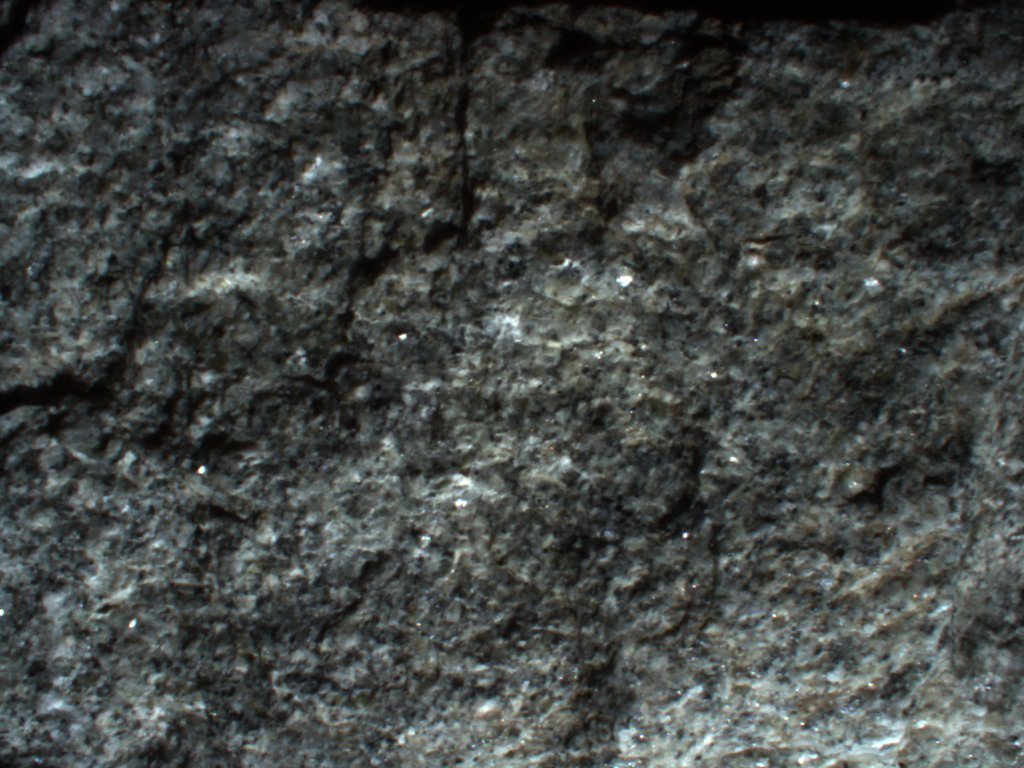
\includegraphics[scale=.18]{image_eps/orig_some/0.eps}
}
\subfigure[]{

\includegraphics[scale=.18]{image_eps/orig_some/9.eps}
}
\subfigure[]{

\includegraphics[scale=.18]{image_eps/orig_some/10.eps}
}
\subfigure[]{

\includegraphics[scale=.18]{image_eps/orig_some/26.eps}
}
\label{fig:3dtexture} 
\caption{Variation in appearance of the same surface
patch, when illuminated from different lighting directions}
\subfigure{
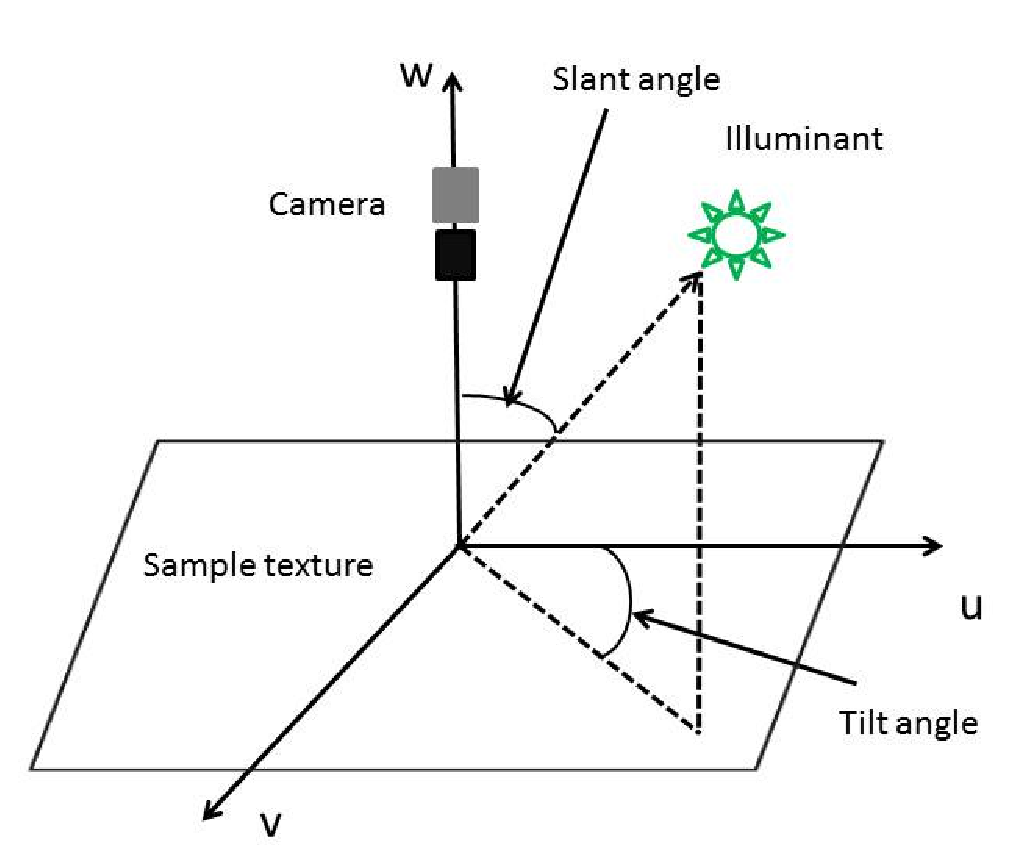
\includegraphics[scale=.58]{chap3/res_2/setup.eps}
}
\label{fig:setup}
\caption{Experimental setup}
\end{figure}
%\begin{figure}[t]
%\centering

%\label{fig:figure1}
%\end{figure}
%\begin{figure*}[t]
%\centering

%\end{figure*}
% However, the images mapped using this technique
%exhibit the properties of the lighting condition in which they were captured.
Mapping 2D textures or images is the most common method used, which is
efficient for most 3D models and scenes, especially where the lighting
conditions remain constant. They look best when the object is viewed in similar lighting conditions as
when the texture is captured. They appear flat and smooth.
In practice, the real world surfaces are
characterized by phenomena such as inter-reflection, self-shadowing, subsurface
scattering, specularity, etc. These properties interact with different lighting
directions and therefore the same surface appears different under
different lighting condition Fig 1.2. 2D texture fails to capture these complex reflectance properties of a 
surface and therefore a rendered surface looks highly unrealistic in case the lighting
conditions are changed. In order to produce a realistic rendering it is necessary to capture
and model the interaction of the material surface with different lighting
conditions. \cite{C1} investigates the problem of representation, recognition, synthesis of
natural materials and their rendering under arbitrary viewing/lighting conditions.

%They only model the reflectance properties of a surface,
%which alone is not sufficient for a realistic rendering of the real world
%materials. 



%%%%%%%%%%%%%%%%%FIGURE NO 1%%%%%%%%%%%%%%%


3D textures are a way to model this relation between surface reflectance
properties and illumination/viewing conditions.
The use of 3D texture modeling
results in enhanced realism of the scene. Reflectance texture maps are one of
the techniques that can be used to compactly represent the 3D textures. These
maps are generated using image re-lighting techniques \cite{C5,C4,C2} in which
multiple images are captured under different lighting conditions.

%Bidirectional Reflectance Distribution Function\cite{B1}, which defines the
%spectral and reflectance characteristics of a surface can be used to create
%reflectance texture maps. It is defined as the ratio of reflected radiance to
%incident irradiance, given the lighting and viewing directions. The reflectance
%at each point on a surface is hence a function of four parameters, controlling
%the above two directions. Various techniques have been developed to compactly
%represent BRDF \cite{B5,B8,B12,B14,B15}. It was extended to Bidirectional
%Texture Function \cite{B2} by allowing BRDF to vary spatially across planar
%texture co-ordinate (u,v).

%3D Texture modelling is an important area in computer graphics as it results in realistic rendering
%of natural material surfaces.The characterization of surface reflectance properties is important in
%achieving photorealism.The appearance of a surface in different lighting and viewing direction/
%conditions is affected by its reflectance properties.3D texture actually models the relation
%between surface reflectance properties and illumination direction. They are represented
%by Reflectance Texture Maps.These maps are generated using image re-lighting techniques
%\cite{B2,B6,B13} which model the surface reflectance properties of object.

%2D texture modelling fails to capture the surface variation and reflectance properties under
%varying lighting and viewing direction.They appear good only when viewed from similar lighting
%direction in which they were captured.2D textures appear flat and smooth but reflectance properties
%of real world objects are characterised by inter-reflections,shadows,specularity and sub-surface
%scattering. 2D texture fails to provide the information required for rendering other than the original
%illumination condition. Figure 1 illustrates how  the same texture behaves differently under different lighting conditions.

%It is clear from thefigure that 2D texture which has only the color information alone is not sufficient for a realisitic
% rendering of real world texture
%and therefore 3D texture is needed.

%Reflectance map required in 3D texture can be modelled by Bidirectional Reflectance Distribution
%Function \cite{B1} technique which defines spectral and spatial reflectance characteristic of a
%surface.BRDF is the ratio of reflected radiance to incident irradiance.Various techniques have been
%developed to compactly represent BRDF \cite{B5,B8,B12,B14,B15}.

%BRDF was extended to Bidirectional Texture Function \cite{B2} by allowing BRDF to vary spatially
%across planar texture co-ordinate (u,v)

%\begin{equation}
%BTF=(\theta_{v},\phi_{v},\theta_{e},\phi_{e},u,v)
%\end{equation}


%BTF effectively captures view point dependent phenomenon such as specularity
%along with other physical phenomenon such as shadow, sub-surface scattering,
%inter-reflection, etc. However, the capture of BTF requires careful camera
%calibration and capturing numerous images for sampling. Generating reflectance
%map from BTF is very complex. View dependent appearances can also be modeled
%using Light field maps \cite{B18}. They offer a more compact representation and
%can be used for a real time rendering of surface light fields.

%Because of the  high dimensionality of the BTF and high storage requirement,
%Unidirectional Texture Functions (UTF) were introduced in which viewing point is
%not taken into account while modeling the surface reflectance properties. They
%model these properties only in relation to different lighting conditions. As the
%visual appearance of the surface is mostly independent of the viewing direction,
%the model provides a reasonable approximation of the surface with significantly
%lower complexity of the model.

Image based modeling techniques \cite{C8,C6,C7} have emerged as
an effective approach for realistic rendering of 3D objects,
where multi-view geometry is utilized in directly synthesizing 
an unseen view of an object from nearby views without
explicit surface reconstruction. The traditional object models capture the shape information in the meshes,
while the reflectance and the surface properties are relegated in the textures. 3D models such as 
Polynomial Texture Maps (PTM) capture the 
surface properties more faithfully, including the effect of small scale height variation on the surface.

Polynomial Texture Maps \cite{C4} belong to the class of UTFs (Uni-directional Texture Function). It is a pixel
based technique that concisely models the surface reflectance properties using a
polynomial model for the reflectance, dependent on two angular parameters of the
lighting direction ($l_u$ and $l_v$). PTMs reconstruct the color of the surface under varying
lighting conditions and models real world phenomenon such as
self-shadowing, inter-reflection and sub-surface scattering. They thus introduce
enhanced photorealism in texture mapping.
Polynomial Texture Mapping is applied in a wide
range of archaeological contexts \cite{C14}. 
It also offers advantages over traditional raking
light photography for examining and
documenting the surface texture and
shape of paintings \cite{C13}.
Recently, PTMs have been used in cultural heritage field to document and virtually inspect 
several sets of small objects, such as cuneiform tablets and coins.


%In the following section we
%summarize the results of our recent applications in conservation
%recording and comparison, analysis of archaeological materials,
%archaeological representation and dissemination.


%\subsection{3D texture VS 2D texture}

%In 2D texture modelling,the reflectance and the strutural properties of natural surfaces
%are not captured.They fail to capture the variations in surfaces for different lighting and
%viewing directions.In ed texture mapping the texture which is mapped onto a 3d model has
%the lighting direction from which it was captured.So if we want to see how the texture looks from
%different lighting direction,this mapping will give poor results when viewed from different
%lighting direction apart from the direction from which it was captured.In general,Real world objects
%are not flat and smooth in nature.They show different types of structural variation across their
%surface each having different reflectance properties.These properties causes effects like shadows,
%specularity sub-surface scattering,inter-reflection etc.Hence 3d texture mapping
%is required for realisting modelling of real objects.

%\subsection{BRDF}

%Reflectance texture maps are compact model for representing 3d textures.They model the spatial
%variation in surface luminance as a function of viewing and illumination direction.
%The bidirectional reflectance function \cite{A3} characterizes the color of a surface as a function
%of incident light and view directions.

%The BRDF is the ratio of the reflected intensity in the exitant direction to the incident
%energy per unit area along the incident direction.

%\subsection{PTM}
%Polynomial Texture Maps \cite{A1} is a pixel based technique used to model luminiance
%against changing lighting direction.PTMs reconstruct the color of a surface under varying lighting
%conditions. When a surface is rendered with a PTM, it takes on different illumination
%characteristics depending on the direction of the light source.

%PTM model uses a set of input images captured from a fixed camera, where each
%image is illuminated from a specific known lighting direction. It uses a
%biquadratic polynomial function with 6 coefficients per pixel for modeling the
%reflectance. These coefficients are estimated from the set of input images(30 to
%40), where the lighting direction is resolved into two components i.e
%$l_{u}$,$l_{v}$ by projecting it on the image plane. These two components are
%used as variables in the biquadratic function. Once the coefficients are
%estimated fitting the model to the observed values, they are used to render
%images from any given lighting direction.



\subsection{Problem}
Texture mapping is an important area in computer graphics which adds realism to three dimensional models.
2D texture mapping fails to capture the surface variation and reflectance properties under
varying lighting and viewing direction. They appear good only when viewed from similar lighting
direction in which they were captured and fails to provide the information required for rendering other than the original
illumination condition. But 3D textures correctly models the relation between surface reflectance
properties and illumination conditions.The use of 3D texture modeling
results in enhanced realism of the scene.

PTM technique causes overall smoothening of light which dampens the effect
of specularity and softens sharp shadows. The effect of point light source is
reduced and the appearance is always similar to a diffused light source.
Therefore we improve upon the PTM model 
to overcome the above limitations
and generate a complete 3D Texture model that can be evaluated at individual
pixels. We propose an approach to image-based lighting interpolation that is
based on estimates of geometry and shading from a set of input images.
%The current state-of-the art
%in the field of PTM involves robust method for interpolation of shadow and specularity,Drew {\em et al.}\cite{A10} 
%But they do not model natural material surfaces and their interactions
%with changing light conditions.
%Moreover the number of per pixel parameters are too high for real-time rendering. 
%\cite{A3} shows that surface normals
%extracted from the PTM image data structure are of lower
%quality because of the smoothing caused by the use of biquadratic function, which compromises the directional 
%accuracy of the normals.
%PTM. The directional accuracy of the normals is compromised
%by the PTM biquadratic function’s smoothing over the range of
%illumination angles in the hemisphere


\begin{figure*}[t]
\centering
%\subfigure[]{
\includegraphics[height=3.7in,width=6.2in]{sep_images/sep3.eps}
%\label{fig:subfig23} } \caption[] {Components of a sponge image: a) Original image, b) Direct c) Global
%component.} 

\caption{Component Based Modeling (CBM)}
\label{fig:CBM}
\end{figure*}

\subsection{Approach}
We capture multiple images of a static object with a static camera under varying
lighting conditions.
The scene is
illuminated using a high frequency checkerboard pattern using the projector. The
projector is moved to different lighting positions for the purpose of obtaining
images with different lighting directions. Experimental setup is shown in Figure \ref{fig:setup}

When we separate the image of the texture into direct and the global part, we find
that the shadows and the specularities appear very strongly in the direct part,
as these are phenomena that involve light that reaches the surface point
directly from the light source. The fine details and the structure of the
material are very prominently visible in the direct part as they are observed
primarily through shadows. On changing the lighting direction, the change in the
luminance of the direct part is minimal as long as the surface point is directly
illuminated. The variations are introduced, primarily by self-shadowing and
specularity, both of which are abrupt changes as the lighting direction changes.
The global component contains the lighting of a surface point from other
parts in a scene, and hence it captures the overall illumination as well as
color variations of a surface with lighting direction. As the lighting direction
changes, the luminance value of the global part varies significantly.

Both direct and global components are separately analyzed to derive the
corresponding models and parameters. Given a new lighting direction, we use the
two models separately to generate the corresponding components, and combine them
to get the final image. Then for a new lighting direction, we can readily
interpolate both specular content as well as shadows.
The main contributions of this work are (1) Direct and Global modeling characterized by
shadows, specularity and luminance, 
(2) separate modeling and hence better capturing of shadows and specularities 
and (3) per pixel function model to
achieve real-time rendering of enhanced 3D textures on GPU.
% We decompose images captured at different lighting conditions into intrinsic image
% components; i.e, the {\em direct} and {\em global} image components. Each of
% these components is then further separated to obtain different physical
% phenomena such as shadows, specularity and luminance. The final image is obtained
% by combining the individual models together.
The method is shown to indeed
generate better results for non-observed lighting directions.
A complete flowchart of our model is shown in Fig \ref{fig:CBM}


\section{Analysis of Text in Scene Images}
\begin{figure*}[t]
\centering
\subfigure{
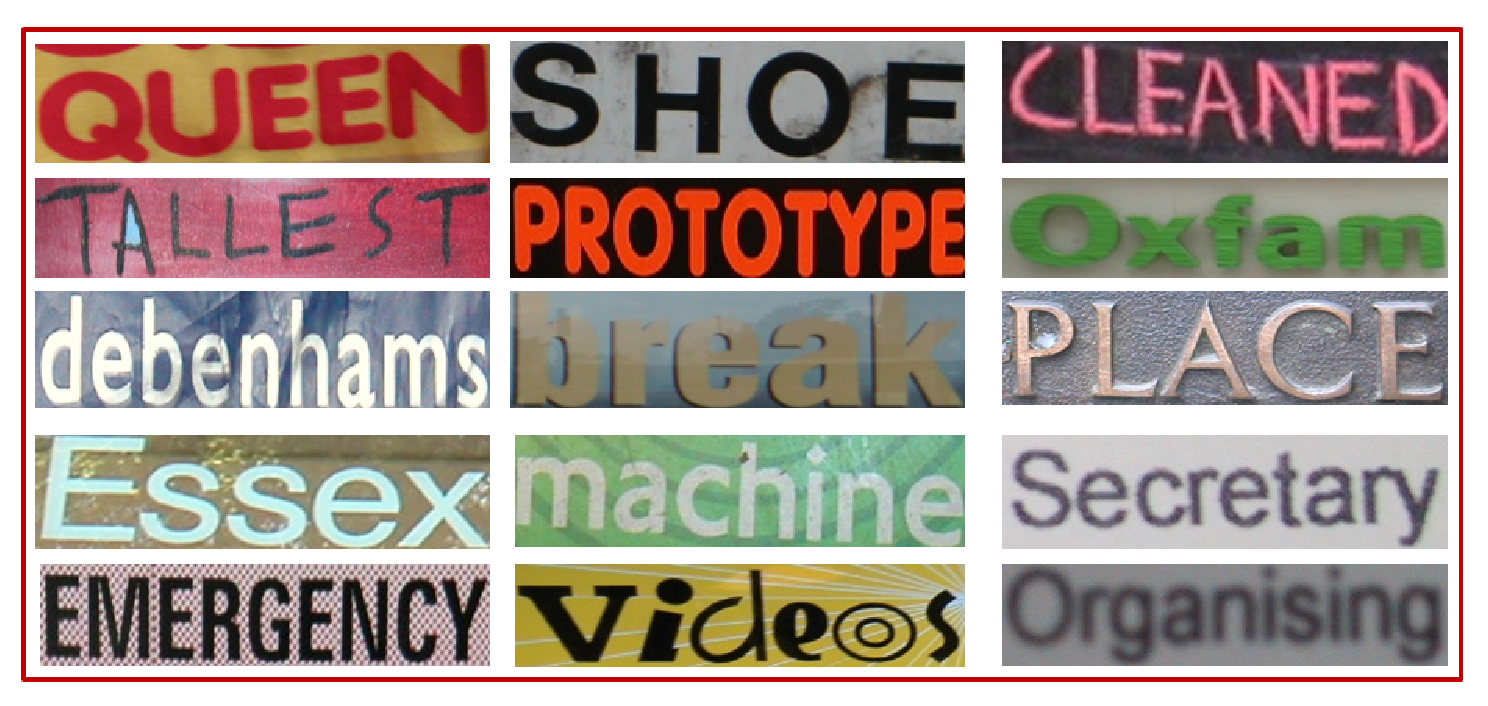
\includegraphics[height=3.6in,width=5.8in]{chap4/res_7/scene_text.eps}
}
\caption
{Natural Scene Text Images}
\label{fig:scenetext}
\end{figure*}
\begin{figure*}[t]
\centering
\subfigure{
\includegraphics[height=4.1in,width=5.5in]{chap4/res_7/text_chall.eps}
}
\caption
{Scene text images containing complex background}
\label{fig:textchallenge}
\end{figure*}

Scene text is textual content that is captured by a camera in an image.
Reading text captured in images provides valuable information and is
used in many content-based image
applications such as content based web image search,
information retrieval and mobile based text analysis
and recognition.

In the recent years, content-based image analysis techniques have received more attention with the 
advent of various digital image capture devices.
Applications of text localization
and recognition in real-world images ranges widely. It is used for indexing large image/video
databases by their textual content, sign recognition
for foreigners, automatic license plate recognition, assisting the elderly and visually
impaired in reading labels.

The images captured by these devices can vary dramatically depending on lighting conditions, reflections, 
shadows and specularities. Some natural scene text images are shown in Fig \ref{fig:scenetext}.
These images contain numerous degradations such as uneven lighting, complex background, multiple colours, blur etc.
We propose a method which removes reflections, shadows and specularities from natural scene text images and 
binarizes the text from a single image.
Binarization method is one of the important pre-processing steps in document image analysis system. 
It directly affects the performance of the subsequent step which is text recognition.
Binarization of text can be defined as classifying individual pixels as foreground (text) or background. 

There are many algorithms that aim at extracting foreground text from background in images but thresholding remains one of
the oldest form that is used in many image processing applications. Many sophisticated approaches often have thresholding as a pre-processing step. 
It is often used to segment images consisting of bright objects against dark backgrounds or vice versa \cite{A1,A3,A4}.
It typically works well for images where the foreground and background are clearly defined.
For color thresholding images, most algorithms convert the 
RGB image into grayscale but here we will make use of the RGB channels as three different sources/components. 

Traditional thresholding based binarization can be grouped into two categories: the one which uses global
threshold for the given images like Otsu \cite{A2}, Kittler {\em et al}. 
\cite{A5} and the one with local thresholds like Sauvola \cite{A6},
Niblack \cite{A9}. In global thresholding methods \cite{A2,A7}, global thresholds are
used for all pixels in image. These methods are fast and robust as
they use a single threshold based on the global histogram of the gray-value pixels of the image.
But they are not suitable for complex
and degraded scene images. 
Also selecting the right threshold for the whole image is usually a challenge 
because it is difficult for the thresholding
algorithm to differentiate foreground text from complex background.

On the other hand, local or adaptive binarization \cite{A8} methods changes the threshold over the image according to local region properties.
Adaptive thresholding addresses variations in local intensities throughout the image.
In these methods, a per-pixel threshold is computed based on a local window around each pixel. 
Thus, different threshold values are used for different parts of the image. 
These methods are proposed to overcome global binarization drawbacks but they can be sensitive
to image artifacts found in natural scene text images like shadows, specularities and reflections.
On the other hand, we propose a method that removes shadows, specularity and reflections and thus produces a clean 
binary images even for the images with complex background.
\begin{figure*}[t]
\centering
\subfigure{
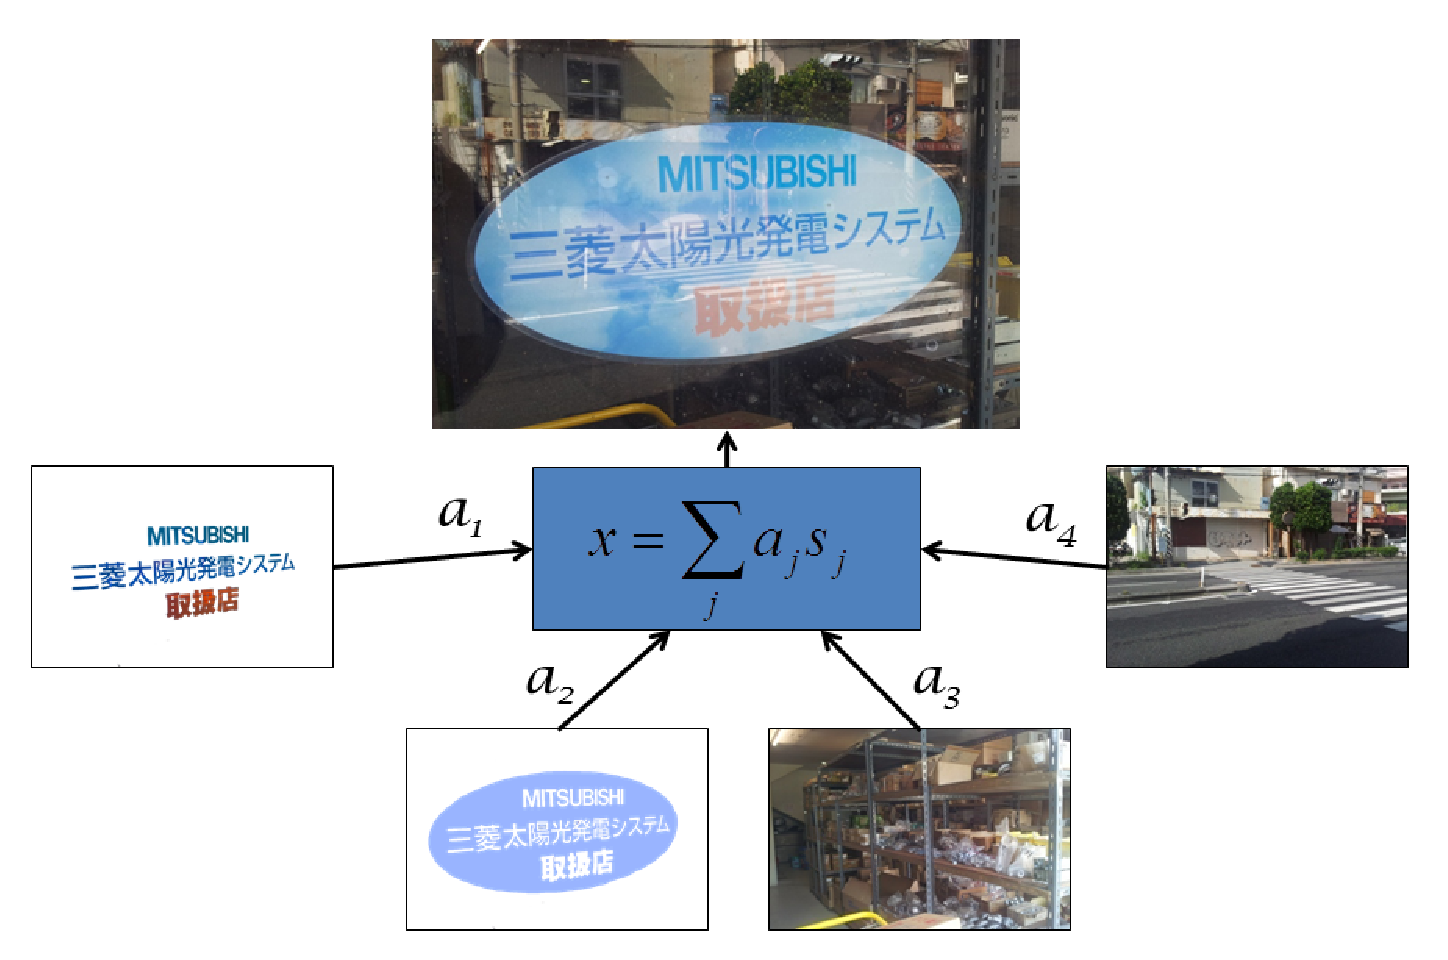
\includegraphics[height=3.8in,width=5.2in]{chap4/res_7/ica_model.eps}
}
\caption
{ICA model applied on images}
\label{fig:ICAmodel}
\end{figure*}
\subsection{Problem}
The primary issue related to segmenting text from scene images is the presence of complex/textured background. 
Some of the challenges are described below:
\begin{itemize}
\item \textbf{Noise:} Sensor noise in handheld camera devices is usually high.
\item \textbf{Viewing Angle:} While capturing images, the text and the camera device may not be parallel.
\item \textbf{Blur:} Some motion blur can
appear or be created by a moving object. Camera shake with hand-held shots can result in blurry images.
Camera not equipped with auto-focus also blurs the image.
\item \textbf{Resolution:}Depending on the capture device, resolutions of the images can vary from low to high.
\item \textbf{Non-planar surfaces:} Text written on non-planar objects like bottles can suffer from deformation.
\item \textbf{Low contrast:} It is difficult
to extract text when there is not much color difference between the foreground text and the background.
 \item \textbf{Lighting:}
Images containing uneven lighting, reflections, shadowing, highights make colors of the text vary drastically and thus 
decreases analysis performance.
Both the physical environment and uneven response/artificial lighting from the camera devices are responsible for 
complexing the task of text extraction.
\end{itemize}
Some of the challenges that we encounter while segmenting natural scene text are shown in 
Fig \ref{fig:textchallenge}.

\subsection{Approach}
We apply an Independent Component Analysis (ICA) model on natural scene images.
It is one of the most important methods of blind source separation and has received  
attention in the field of signal processing, pattern recognition, data compression and image analyzing.
Using ICA,  we can extract the source signals from the 
observations based on the stochastic property of the input signals/images
even without any information of the original source signals.  
ICA method obtains features that present the data through a set of 
components that are statistically independent and characterizes the data 
in a natural way. 
ICA based decomposition enables us to separate text from complex backgrounds containing, reflections,
shadows and specularities. Fig \ref{fig:ICAmodel} shows the basic ICA model applied on images.
For binarization, we apply a global thresholding method on the independent components of the image
and that with maximum textual properties is used for extracting the foreground text. Binarization results show 
significant improvement in the extraction of text over other reported methods. 




\section{Outline}


In this chapter, we briefly analysed textures and text in scene images. 
The rest of this thesis is organized as follows: 
We will survey techniques related to texture mapping and scene text understanding in Chapter 2. In Chapter 3
component based texture modeling will be discussed where we will show how each component is
modeled differently to achieve photorealism.
In Chapter 4, we will discuss component based text segmentation from natural scene images. Finally we 
conclude the thesis summarizing our main contributions and discuss future work in Chapter 5.


%This thesis is organized in four main parts. In the first part in Chapter-1, we give a brief introduction
%on biometrics and fingerprints. We talk about various biometric traits such as face, iris, hand geometry
%etc and see why fingerprints are the most popular and widely used in biometric authentication systems
%around the world. Then, we have a look at the structure of a fingerprint at a global level and at a
%local level. We look at the functioning of a fingerprint recognition system in verification mode and in
%identification mode. Readers who are familiar with biometrics and functioning of fingerprint recognition
%systems can skip this chapter and move on to the second part. In the second part in Chapter-2, we discuss
%about the problem of matching two fingerprints. We talk about matching using global features such as
%core points, ridge structure etc and see how matching at a local level using minutiae-based features
%leads to a better accuracy. We do an exhaustive survey on minutiae-based local fingerprint matching
%techniques. Most of these techniques build local minutiae structures from invariant distances and angles
%in the neighborhood of each minutia. We have a look at existing local structures and their weaknesses
%and lay motivation for a new local minutia structure. Then in the third part in Chapter-3, we look at the
%problem of fingerprint identification over a large database. We propose a new minutiae structure called
%an Arrangement Vector that describes the geometric arrangement of neighboring minutiae points around
%a central minutia. We propose a hash-based novel indexing mechanism using arrangement vectors and
%show its effectiveness. In the last part of thesis (Chapter-4), we extend the Arrangement vector into a
%fixed length binary representation for a fingerprint and tackle the problem of fingerprint matching. We
%finish this thesis in Chapter-5 by summarizing our main contributions and the directions in which we
%can extend our work.


% Texture mapping adds realism details to raster images with relatively small increase in
% computation and has long been used in computer graphics. Texture can be defined in the
% usual sense (such as cloth, wood, brick and so on), more specifically a detailed pattern or a
% multidimensional image that is mapped into a multidimensional space. In the latter form,
% a photograph is used to map onto a planar surface, which avoids modeling complex surface
% details. However this method fails when the lighting conditions of the synthetic environment
% are different from those of the texture image and the results will look unrealistic and flat [17].
% Due to these problems, the field of image based modeling and rendering (IBMR) has
% attracted people's attention in recent decades. IBMR methods rely on a set of two dimen-
% sional images as inputs. In order to obtain photorealistic rendering, one should be able to
% characterize surface reflectance properties such as surface normal and albedo.

% Texture refers to a surface characteristic and appearance of an object given by
% its geometry, density and surface reflectance, and the stochastic variation of
% these parameters. It also provides a rich source of information about the
% natural scene and hence is important cue in trying to achieve photo realistic
% rendering of 3D models by adding surface details or color to an object or a
% scene. For example, planar walls can have stone textures mapped onto them for a
% very convincing and realistic image of a three dimensional stone wall.

% Mapping 2D textures or images is the most common method used, which is both
% efficient effective for most 3D models and scenes, especially where the lighting
% condition remain constant. However, the images mapped using this technique
% exhibit the properties of the lighting condition in which they were captured.
% Hence they look best when the object is viewed in similar lighting conditions as
% when the texture is captured. In practice, the real world surfaces are
% characterized by phenomena such as inter-reflection, self-shadowing, subsurface
% scattering, specularity, etc. These properties interact with different lighting
% directions conditions and therefore the same surface appears different under
% different lighting condition(see Figure 1).
% 
% 2D texture fails to capture these complex reflectance properties of a surface
% and therefore a rendered surface looks highly unrealistic in case the lighting
% conditions are changed. They only model the reflectance properties of a surface,
% which alone is not sufficient for a realistic rendering of the real world
% materials. In order to produce a realistic rendering it is necessary to capture
% and model the interaction of the material surface with different lighting
% conditions.


%%%%%%%%%%%%%%%%%FIGURE NO 1%%%%%%%%%%%%%%%





%----------------------------------------------------------------------
%\section{First Section} 
%\label{sec:SECTION1NAME}

%Text of section 1 goes here... \\

%This is to insert a table \\

%\begin{table}
%\begin{center}
%\begin{tabular}{|l|c|}
%\hline
%Method & Frobnability \\
%\hline\hline
%Theirs & Frumpy \\
%Yours & Frobbly \\
%Ours & Makes one's heart Frob\\
%\hline
%\end{tabular}
%\end{center}
%\caption{Results.   Ours is better.}
%\end{table}

%This is to insert a figure \\

%\begin{figure}[h]
%\centering
%
\includegraphics[height=2cm,width=0.2\linewidth]{figures/iiit.eps}
%\caption{Analysis of our method}
%\label{}
%\end{figure}



%----------------------------------------------------------------------
%\section{Second Section} 
%\label{sec:SECTION2NAME}

%Text of section 2 goes here... \\

%{\bf Few suggestions}

%-------------------------------
%\subsection{Mathematics}

%Please number all of your sections and displayed equations.  It is
%important for readers to be able to refer to any particular equation.  Just
%because you didn't refer to it in the text doesn't mean some future reader
%might not need to refer to it.  It is cumbersome to have to use
%circumlocutions like ``the equation second from the top of page 3 column
%1''.  (Note that the ruler will not be present in the final copy, so is not
%an alternative to equation numbers).  All authors will benefit from reading
%Mermin's description of how to write mathematics (see math.pdf).


%------------------------------
%\subsection{Footnotes}

%Please use footnotes\footnote {This is what a footnote looks like.  It
%often distracts the reader from the main flow of the argument.} sparingly.
%Indeed, try to avoid footnotes altogether and include necessary peripheral
%observations in 
%the text (within parentheses, if you prefer, as in this sentence).  If you
%wish to use a footnote, place it at the bottom of the column on the page on
%which it is referenced. Use Times 8-point type, single-spaced.

%--------------------------------
%\subsection{References}

%List and number all bibliographical references in 9-point Times,
%